\section{1174035 - Luthfi Muhammad Nabil}

\subsection{Teori}
    \begin{enumerate}

        \item Jelaskan dengan ilustrasi gambar sendiri apa perbedaan antara vanilla GAN dan cGAN.
		Vanilla GAN merupakan sebuah metode GAN standar yang menjadi basis dari metode GAN lainnya. VanillaGAN menggunakan label sebagai peningkat performa dari pelatihan data. Sedangkan Conditional GAN menggunakan label untuk mendiskriminasi dan menghasilkan gambar yang lebih baik.
			\begin{figure}[H]
            	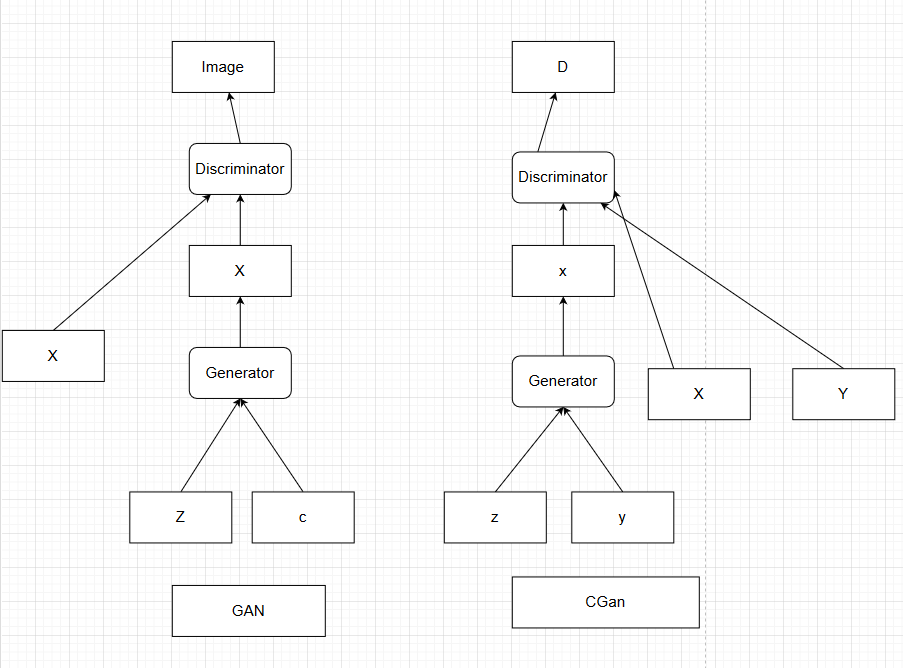
\includegraphics[width=4cm]{figures/1174035/chapter9/teori1.png}
           		\centering
           		\caption{Valina GAN-cGAN}
            \end{figure}
            
        \item Jelaskan dengan ilustrasi gambar sendiri arsitektur dari Age-cGAN.
			Age cGan melakukan input sesuai dengan wajah beserta umur. Lalu akan dilakukan proses encoding dan selanjutnya melakukan Optimasi identitas. Lalu dihasilkan rekonstruksi awal yang nanti dilanjutkan dengan generator yang mengoptimasi rekonstruksi.
			\begin{figure}[H]
				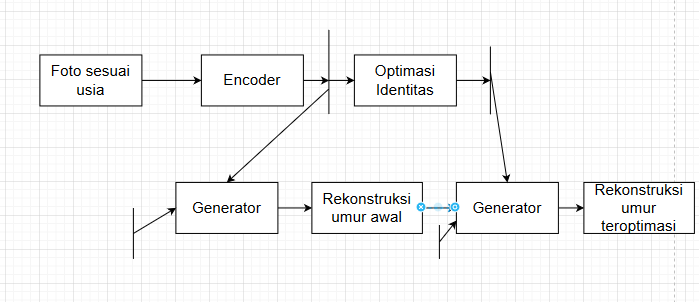
\includegraphics[width=4cm]{figures/1174035/chapter9/teori2.png}
            		\centering
           		\caption{Age-cGAN}
            \end{figure}
                
        \item Jelaskan dengan ilustrasi gambar sendiri arsitektur encoder network dari Age cGAN.
			Encoder network pada Age cGAN menghasilkan vektor dari gambar yang dimasukkan. Encoder network sendiri merupakan sebuah CNN yang mengambil gambar dengan dimensi sekitar 64,64,3 dan mengkonversikannya menjadi vektor dengan dimensi 100
            \begin{figure}[H]
                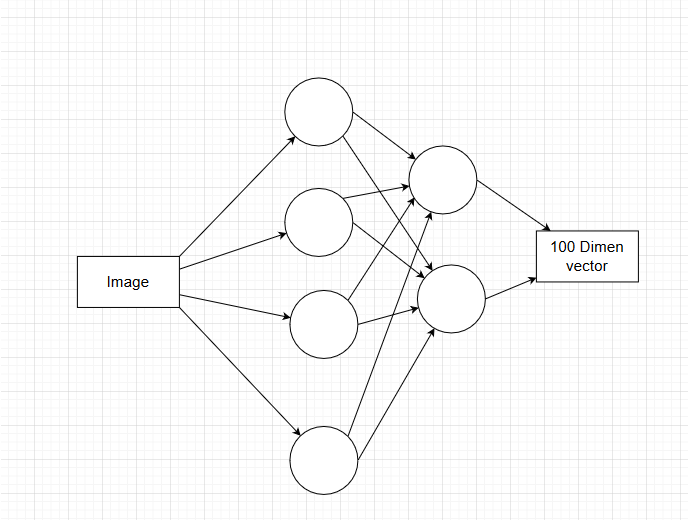
\includegraphics[width=4cm]{figures/1174035/chapter9/teori3.png}
                    \centering
                \caption{Encoder Age cGANr}
            \end{figure}

        \item Jelaskan dengan ilustrasi gambar sendiri arsitektur generator network dari AgecGAN.
		Generator network mengambil representasi yang tersembunyi dari fotowajah dan kondisi vektor sesuai dengan kondisi yang ada. Generator network sendiri memiliki vektor 100 dimensi dan kondisi vektor Y. 
		\begin{figure}[H]
			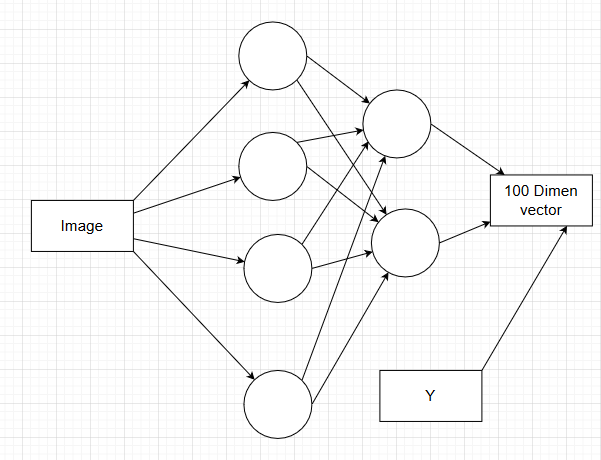
\includegraphics[width=4cm]{figures/1174035/chapter9/teori4.png}
            	\centering
           	\caption{Network Age cGAN}
       	\end{figure}


        \item Jelaskan dengan ilustrasi gambar sendiri arsitektur discriminator network dari Age-cGAN.
		Arsitektur diskriminator arsitektur yang mampu menerima input gambar dengan ukuran 28,28 serta menghasilkan angka biner yang menyatakan apakah data yang diinputkan merupakan dataset asli atau gambar dataset palsu.
		\begin{figure}[H]
			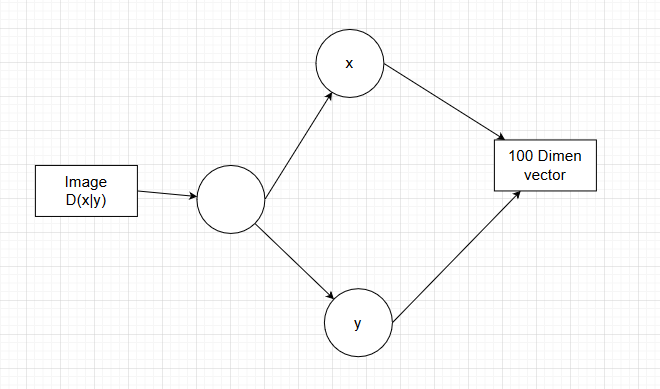
\includegraphics[width=4cm]{figures/1174035/chapter9/teori5.png}
            	\centering
           	\caption{Discriminator Age cGAN}
       	\end{figure}


        \item Jelaskan dengan ilustrasi gambar apa itu pretrained Inception-ResNet-2 Model.
		Inception Resnet 2 model pre trained merupakan sebuah package untuk mendefinisikan, melatih, dan mengevaluasi sesuai dengan checkpoint dan definisi model untuk beberapa network pada klasifikasi gambar.
		\begin{figure}[H]
			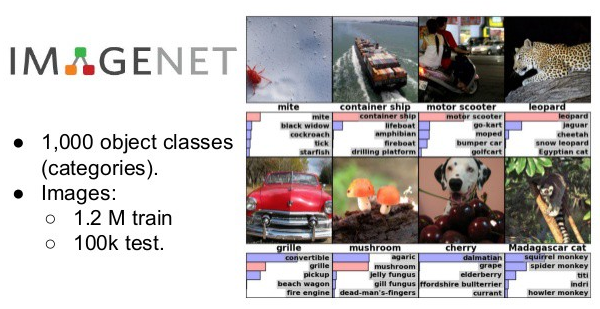
\includegraphics[width=4cm]{figures/1174035/chapter9/teori6.png}
            	\centering
           	\caption{Pretrained Inception ResNet}
       	\end{figure}

        \item Jelaskan dengan ilustrasi gambar sendiri arsitektur Face recognition network Age-cGAN.
        Face recognition akan mengevaluasi sesuai dengan umur yang ada, lalu akan dilakukan sebuah encoding data untuk menghasilkan data yang sesuai. Nanti akan dihasilkan terlebih dahulu data awal lalu dioptimasi data tersebut.
		\begin{figure}[H]
			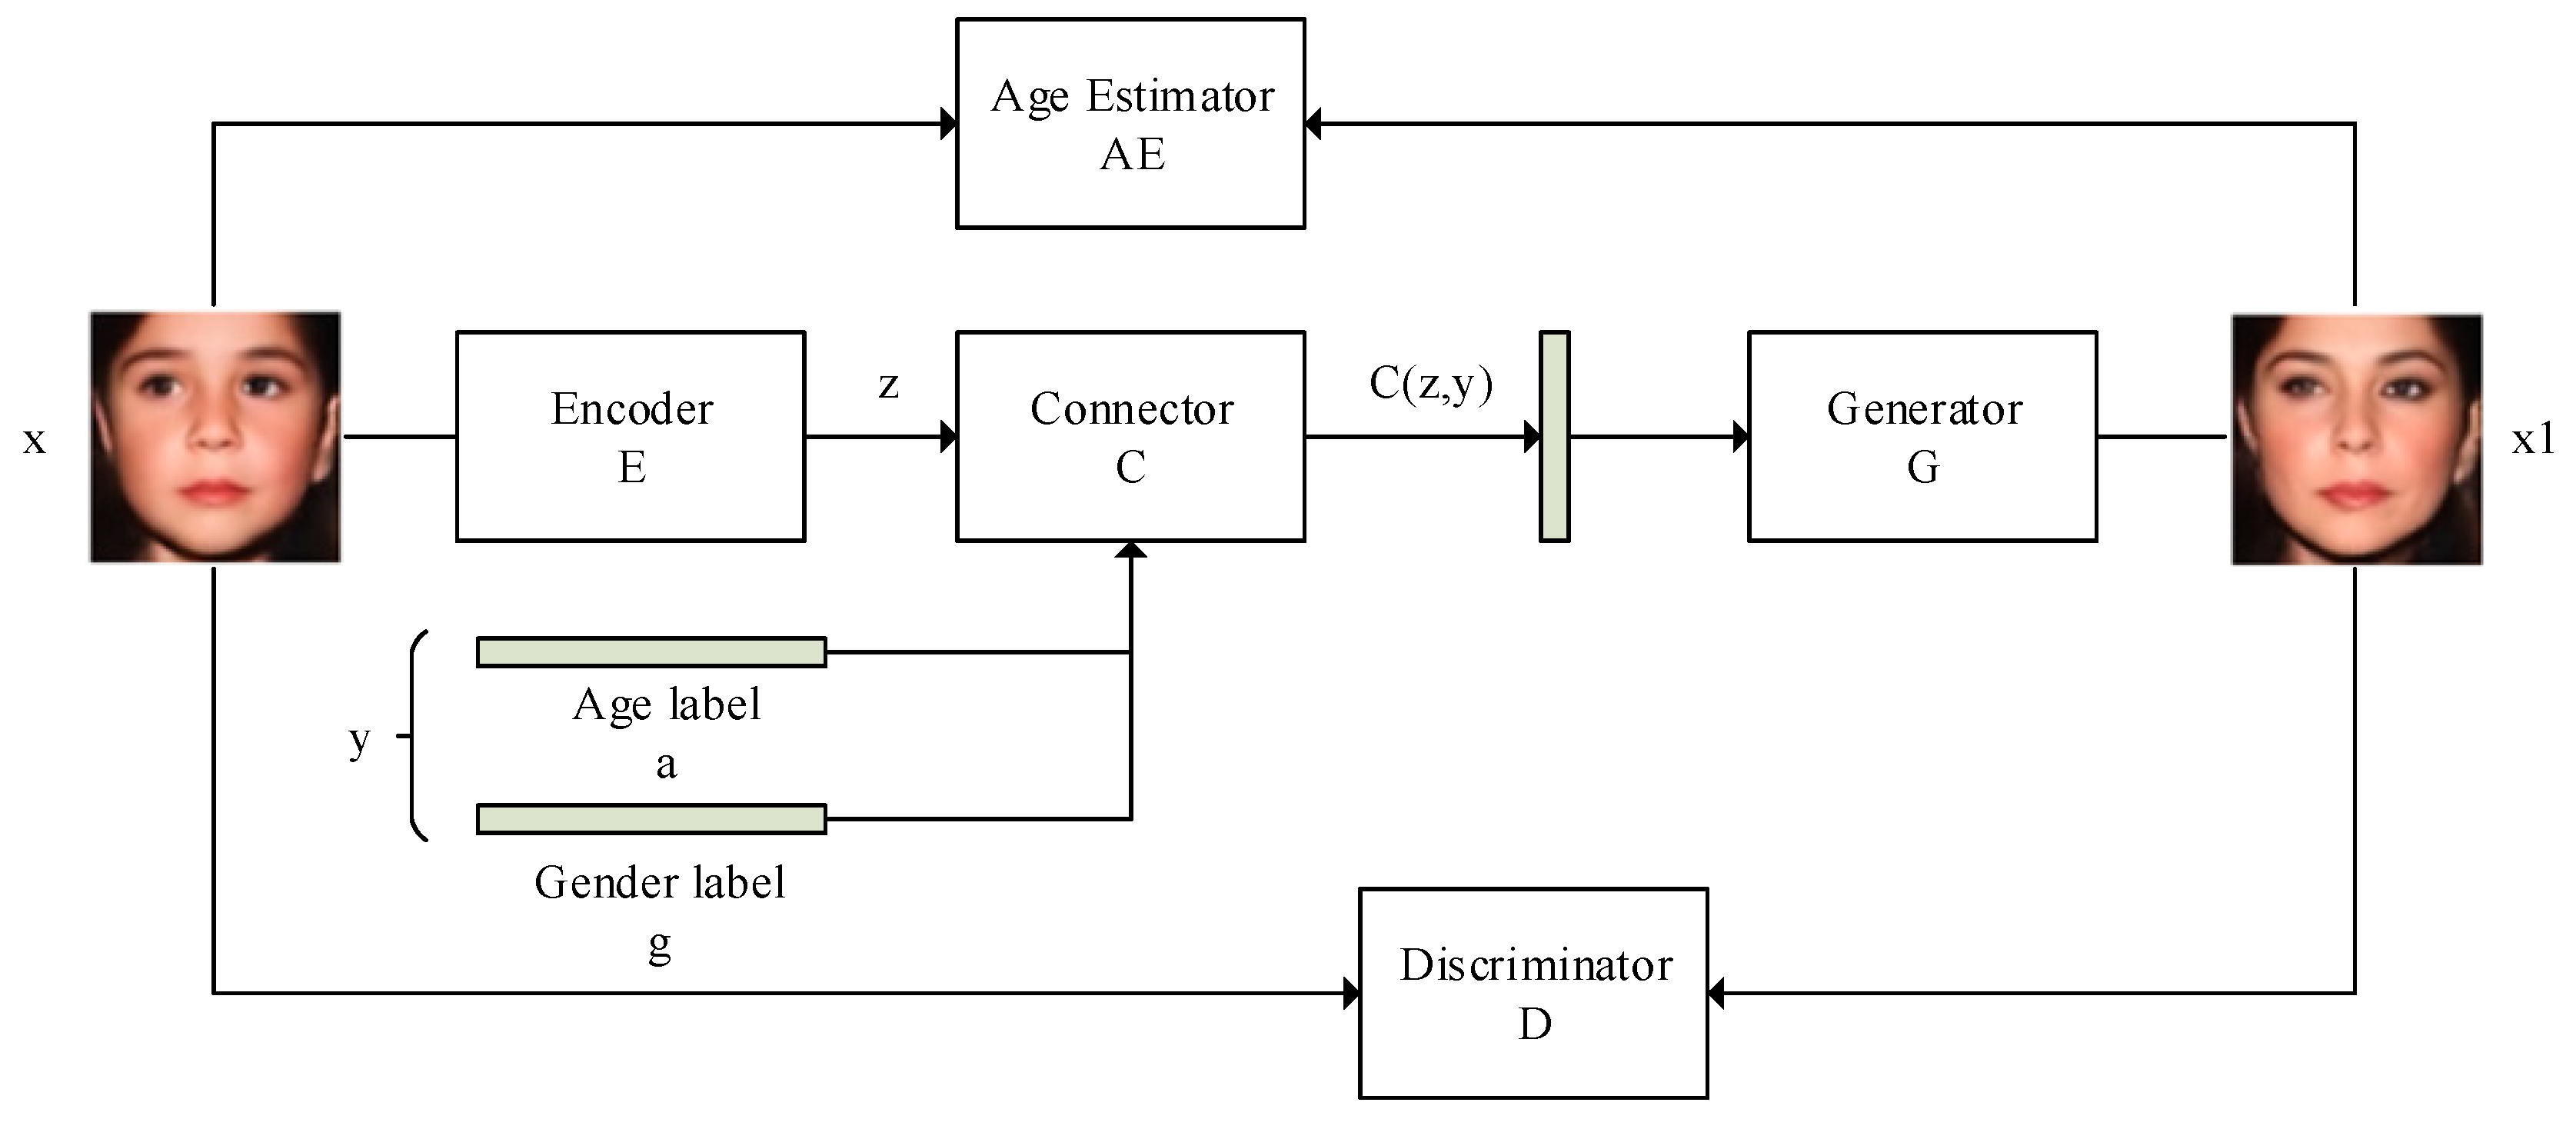
\includegraphics[width=4cm]{figures/1174035/chapter9/teori7.png}
            	\centering
           	 \caption{Face recognition network Age-cGAN}
       	 \end{figure}

        \item Sebutkan dan jelaskan serta di sertai contoh-contoh tahapan dari Age-cGAN.
		Pada dari Age-cGan ni terdapat 2 tahapan dengan generator dan diskriminator. dimana untuk tahap generator sendiri membutuhkan vektor laten 100 serta menghasilkan gambar yang realistis dari dimensinya. sedangkan tahap diskriminator itu tahapan dimana memprediksi gambar yang diberikan nyata atau palsu.
		\begin{figure}[H]
			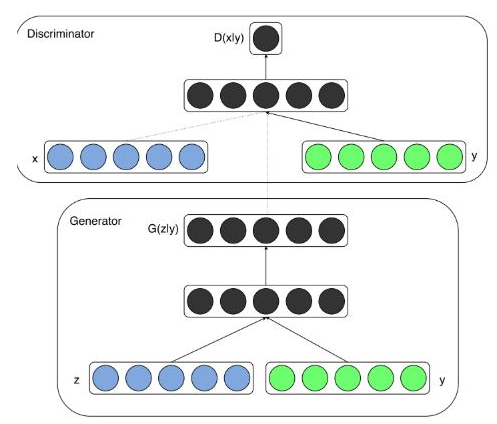
\includegraphics[width=4cm]{figures/1174035/chapter9/teori8.png}
            	\centering
           	 \caption{Tahap Age cGAN}
       	\end{figure}

        \item Berikan contoh perhitungan fungsi training objektif.
		Objektif Trainning ialah untuk meminimalkan loss function sebagai log likelihood function yang diberikan pada persamaan dimana D melambangkan trainning data.
		\begin{figure}[H]
			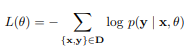
\includegraphics[width=4cm]{figures/1174035/chapter9/teori9.png}
            	\centering
           	 \caption{Training Objektif}
       	\end{figure}

        \item Berikan contoh dengan ilustrasi penjelasan dari Initial latent vector approximation.
		Latent vector approximation menghasilkan sebuah reverse mapping untuk menghasilkan sebuah latent vector yang diukur sesuai dengan perkiraan yang sudah ditentukan.
		\begin{figure}[H]
			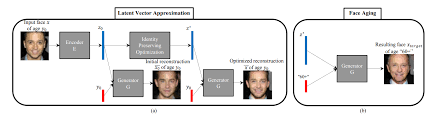
\includegraphics[width=4cm]{figures/1174035/chapter9/teori10.png}
            	\centering
           	 \caption{Initial Latent Vector Approximation}
       	\end{figure}

        \item Berikan contoh perhitungan latent vector optimization.
		Perhitungan lantent optimization menggunakan metode yang relatif sederhana, tergantung pada jumlah kecil parameter yang diperlukan, sehingga pada latent optimization dapat memetakan setiap gambar x dari dataset ke vektor acak dimensi rendah zi dalam ruang laten z.
		\begin{figure}[H]
			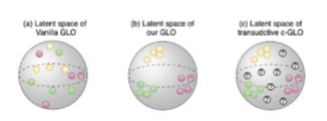
\includegraphics[width=4cm]{figures/1174035/chapter9/teori11.png}
            	\centering
           	\caption{Latent Vector Optimization}
        \end{figure}
           
    \end{enumerate}

\subsection{Praktek}

    \begin{enumerate}
		\item Jelaskan bagaimana cara ekstrak file dataset Age-cGAN menggunakan google colab.
		Menggunakan Google Colab, dimana membuat notebooks baru, kemudian membuat ekstraksi file dari link dataset.
		\lstinputlisting[firstline=1, lastline=4]{src/1174035/chapter9/chapter9.py}

		\item Jelaskan bagaimana kode program bekerja untuk melakukan load terhadap dataset yang sudah di ekstrak, termasuk bagaimana penjelasan kode program perhitungan usia.
		Dibawah ini merupakan code untuk melakukan fungsi perhitungan usia.
		\lstinputlisting[firstline=6, lastline=31]{src/1174035/chapter9/chapter9.py}

		\item Jelaskan bagaimana kode program The Encoder Network bekerja dijelaskan dengan bahawa awam dengan ilustrasi sederhana.
		Proses Encoder berfungsi untuk mempelajari pemetaan terbalik dari gambar wajah dan kondisi usia dengan vector latent Z.
		\lstinputlisting[firstline=33, lastline=73]{src/1174035/chapter9/chapter9.py}

		\item Jelaskan bagaimana kode program The Generator Network bekerja dijelaskan dengan bahawa awam dengan ilustrasi sederhana.
		Proses Generator agar bekerja dengan baik dibutuhkan representasi dari gambar wajah dan vector kondisi sebagai inputan yang menghasilkan sebuah gambar.
		\lstinputlisting[firstline=75, lastline=104]{src/1174035/chapter9/chapter9.py}

		\item Jelaskan bagaimana kode program The Discriminator Network bekerja dijelaskan dengan bahawa awam dengan ilustrasi sederhana.
		Proses Discriminator untuk membedakan antara gambar asli dan gambar palsu.
		\lstinputlisting[firstline=116, lastline=148]{src/1174035/chapter9/chapter9.py}

		\item Jelaskan bagaimana kode program Training cGAN bekerja dijelaskan dengan bahawa awam dengan ilustrasi sederhana.
		Proses Training cGAN ini dengan load file .mat pada dataset lalu epoch sebanuak 500 kali.

		\lstinputlisting[firstline=150, lastline=167]{src/1174035/chapter9/chapter9.py}

		\item Jelaskan bagaimana kode program Initial dan latent vector approximation bekerja dijelaskan dengan bahawa awam dengan ilustrasi sederhana.
		Initial dan Latent Vector Approximation bekerja melakukan predicsi epoch yang telah di buat sebanyak 500 kali, dan nanti hasilnya ada di folder result.

		\lstinputlisting[firstline=169, lastline=217]{src/1174035/chapter9/chapter9.py}

\end{enumerate}

\subsection{Penanganan Error}
\begin{enumerate}
	\item Tidak ada error yang terjadi
\end{enumerate}

\subsection{Bukti Tidak Plagiat}
\begin{figure}[H]
\centering
	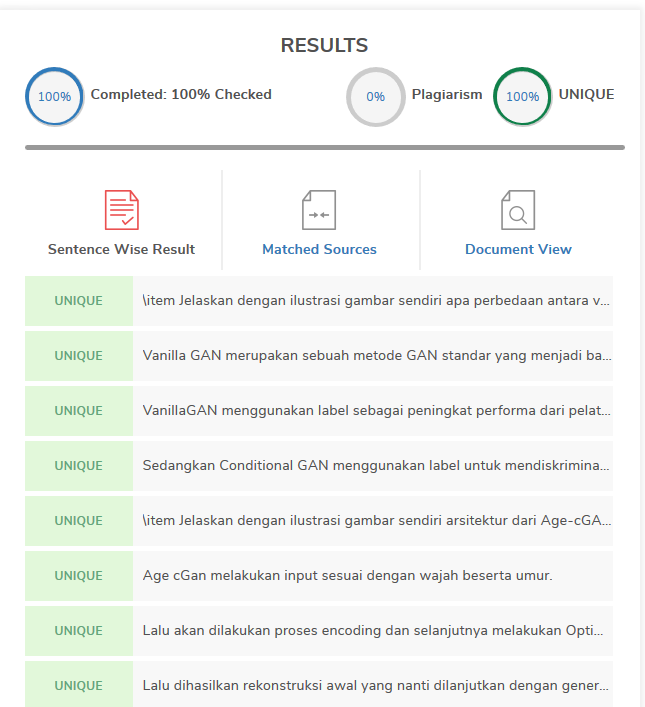
\includegraphics[width=4cm]{figures/1174035/chapter9/plagiat.png}
	\caption{Bukti Tidak Melakukan Plagiat Chapter 9}
\end{figure}